\chapter{Effects of soil microbes on plant competition: a perspective from modern coexistence theory}
%\chaptermark{Positive frequency-dependence}
%\renewcommand{\sectionmark}[1]{}
\fancyhead[LE, RO]{\thepage}
\fancyhead[RE]{CHAPTER 4}
\fancyhead[LO]{SOIL MICROBES AND PLANT COEXISTENCE}
\fancyfoot{}
\renewcommand{\headrulewidth}{0pt}
\setlength{\parindent}{1cm}



\begin{comment}
\documentclass[hidelinks,letterpaper, 11pt]{article}
\usepackage{graphicx, bm, booktabs, lineno, array}
\usepackage[fleqn]{amsmath}
\usepackage{nicefrac}
\usepackage[compress,comma]{natbib}
\usepackage[right=1in, left=1in, top=1in, bottom=1in]{geometry}
\usepackage[parfill]{parskip}
\usepackage[usenames,dvipsnames]{color}
\usepackage[font=large,labelfont=bf,margin=1cm, labelsep = none]{caption} % caption formatting
\usepackage{setspace}
\usepackage{gensymb}
\usepackage{color}
\usepackage{sidecap}
%\usepackage{floatrow}
\usepackage{etoolbox}
\usepackage{tcolorbox}
\usepackage{newpxtext,newpxmath}
\tcbuselibrary{breakable}
%\usepackage{indentfirst}
\newbool{MyRefNumbers}
\usepackage{authblk}
\usepackage{hyperref}
\usepackage{mathpazo}
\usepackage[color=cyan, textsize=tiny]{todonotes}
\usepackage[font={normalsize}]{caption}
\usepackage{adjustbox}
\usepackage{array}
\usepackage{booktabs}
\usepackage{multirow}
\usepackage{tabularx}
% \usepackage{titling}

\setlength{\mathindent}{0pt}
\setlength{\parindent}{1cm}
% \makeatletter
% \makeatother
\pdfminorversion=3

% For table
\newenvironment{myindentpar}[1]%
{\begin{list}{}%
		{\setlength{\leftmargin}{#1}}%
		\item[]%
	}
	{\end{list}}
\newcommand*\samethanks[1][\value{footnote}]{\footnotemark[#1]}
\newcommand\blfootnote[1]{%
	\begingroup
	\renewcommand\thefootnote{}\footnote{#1}%
	\addtocounter{footnote}{-1}%
	\endgroup
}
\newcommand{+}{\raisebox{.4\height}{\scalebox{.6}{+}}}
\newcommand{\minus}{\raisebox{.4\height}{\scalebox{.8}{-}}}
% Command to recount supplement
\newcommand{\beginsupplement}{%
	\setcounter{table}{0}
	\renewcommand{\thetable}{S\arabic{table}}%
	\setcounter{figure}{0}
	\renewcommand{\thefigure}{S\arabic{figure}}%
}
% Command to center oversized images in floats
\newcommand{\centerfloat}{%
	\parindent \z@
	\leftskip \z@ \@plus 1fil \@minus \textwidth
	\rightskip\leftskip
	\parfillskip \z@skip}
\renewcommand\Affilfont{\fontsize{12}{12}\selectfont}
\newcommand{\ignore}[2]{\hspace{0in}#2}
\end{comment}



\begin{comment}
\begin{document}

\doublespacing
\title{Effects of soil microbes on plant competition: \\ a perspective from modern coexistence theory}
\author[* 1]{Po-Ju Ke}
\author[* 1, 2]{Joe Wan}
\affil[1]{Department of Biology, Stanford University, Stanford, California 94305-5020, USA}
\affil[2]{Institute of Integrative Biology, Department of Environmental Systems Science, ETH Z\"{u}rich, 8092 Z\"{u}rich, Switzerland}
\date{}
\maketitle
\blfootnote{* Both authors contributed equally}
\blfootnote{Correspondence author: Department of Biology, Stanford University, Stanford, California 94305-5020, USA. Phone: +1 650-721-1711. Email: pojuke@stanford.edu, jwan@student.ethz.ch}

\onehalfspacing
\noindent \textbf{Type of article:} Concepts and Synthesis\\
\noindent \textbf{Running head:} Soil microbes and plant coexistence\\
% \noindent \textbf{Keywords:} fitness difference, mutualism, niche difference, pathogens, plant--soil feedback\\
% \begin{myindentpar}{1cm}
	\textbf{Words in Abstract:} 233\\
	\textbf{Words in main text:} 7658\\
	% \textbf{Words in text boxes:} 241\\
	\textbf{Number of references:} 65\\
	\textbf{Number of figures:} 5\\
	\textbf{Number of tables:} 1\\
	\textbf{Number of text boxes:} 2\\
% \end{myindentpar}

% \noindent \textbf{Authorship statement:} PJK conceived the study; PJK and JW performed the analysis and wrote the manuscript.\\

% \noindent \textbf{Data accessibility statement:} No original data appear in this manuscript. Should the manuscript be accepted, all computer scripts supporting the results will be archived in an appropriate public repository such as Github, with the DOI included at the end of the article.\\

\doublespacing
\linenumbers
\end{comment}



\section{Abstract}
Growing evidence shows that soil microbes affect plant coexistence in a variety of systems. However, since these systems vary in the impacts microbes have on plants and in the ways plants compete with each other, it is challenging to integrate results into a general predictive theory.
To this end, we suggest that the concepts of niche and fitness difference from modern coexistence theory should be used to contextualize how soil microbes contribute to plant coexistence. Synthesizing a range of mechanisms under a general plant--soil microbe interaction model, we show that, depending on host-specificity, both pathogens and mutualists can affect the niche difference between competing plants.
However, we emphasize the need to also consider the effect of soil microbes on plant fitness differences, a role often overlooked when examining their role in plant coexistence.
Additionally, since our framework predicts that soil microbes modify the importance of plant--plant competition relative to other factors for determining the outcome of competition, we suggest that experimental work should simultaneously quantify microbial effects and plant competition. Thus, we propose experimental designs that efficiently measure both processes and show how our framework can be applied to identify the underlying drivers of coexistence. Using an empirical case study, we demonstrate that the processes driving coexistence can be counterintuitive, and that our general predictive framework provides a better way to identify the true processes through which soil microbes affect coexistence.
\medskip


\noindent \textbf{Keywords:} equalizing mechanisms, fitness difference, Janzen--Connell hypothesis, mutualism, niche difference, pathogens, plant--soil feedback, stabilizing mechanisms



\section{Introduction}
Ecologists have long invoked resource partitioning to explain the coexistence of competing species~\citep{Gause1934, tilman1982}, yet differences in resource use cannot fully account for plant diversity~\citep{Silvertown2004}. As a result, plant community ecologists have broadened their focus beyond plant--plant competition to address how interactions between trophic levels can affect plant coexistence \citep{Chesson2008, Mordecai2011, Lanuza2018, Cardinaux2018}. Growing evidence suggests that plants can influence the performance of both conspecifics and competitors by modifying soil microbial communities, an effect commonly studied under the framework of plant--soil feedbacks \citep{Bever1997, Bever2003}. Differences in the way competing plants interact with soil microbes might promote plant coexistence~\citep{Bever2003, Chung2016}. Alternatively, soil microbes could favor certain plants over their competitors, creating variation in species' relative abundance~\citep{Klironomos2002, Mangan2010} and invasion success~\citep{Reinhart2006, Ke2015}.
\par


% Problem: plant--soil interactions are complicated
The wide range of plant--soil microbe interactions makes it difficult to draw general conclusions about their effects on plant communities. In some systems, soil microbial communities may be predominantly harmful to plants due to high pathogen prevalence, while in other systems, beneficial microbes such as mycorrhizal fungi may play a more important role.
Moreover, the impacts of soil microbes depend on their degree of host-specificity. For example, pathogens can promote plant coexistence if they are host-specific \citep{Bell2006, Yamazaki2008, Bagchi2010} but may reduce plant diversity if a single species suffers greater attack \citep{Mordecai2011}. On the other hand, mycorrhizal fungi can hinder plant coexistence if the dominant species has greater mycorrhizal dependence \citep{Urcelay2003}, but may promote coexistence if they benefit not only their hosts but also their hosts' competitors \citep{Bever2002}.
Further adding to this complexity, plant--soil microbe interactions do not operate in isolation: their effect on coexistence must be considered within the context of plant--plant competition for limiting resources such as light and soil nutrients \citep{Callaway2004, Casper2007, Shannon2012, Crawford2017}. Indeed, variability in experimental results suggests that the relative importance of plant--soil microbe and plant--plant interactions may be highly system-specific \citep{Lekberg2018}. Because of the context-dependency of soil microbial interactions, an important question remains: what are the general conditions under which soil microbes promote plant coexistence?
\par


% Solution: modern coexistence framework
To synthesize the diverse roles that plant--soil microbe interactions play in plant communities, we draw on modern coexistence theory \citep{Chesson1990, Chesson2000, Chesson2008}. This framework uses two quantitative components to link species differences to competitive outcomes.
Niche differences summarize mechanisms that promote coexistence, such as differences in resource use~\citep{Chesson1990} or parasitism~\citep{Chesson2008}. These prevent competitive exclusion by giving each species an advantage when it is rare. On the other hand, fitness differences, such as differences in reproductive output or environmental tolerance, determine the ability of one species to exclude its competitor.
Thus, modern coexistence theory classifies processes mediating coexistence into two general categories: equalizing mechanisms, which decrease fitness differences between species, and stabilizing mechanisms, which increase niche differences between species~\citep{Chesson2000, Adler2007, Hillerislambers2012}.
Since coexistence requires the niche difference to be greater than the fitness difference between the two species, the two components form a common currency for understanding how mechanisms simultaneously affect coexistence.
Moreover, niche and fitness differences can be calculated for mathematical models \citep{Chesson2008} as well as experimental results \citep{Godoy2014, Gross2015, Kraft2015}, providing a quantitative link between empirical results and theoretical perspectives.
\par


% Summary of our goal
Taking advantage of the strengths of modern coexistence theory, we provide a unified framework that predicts and classifies the effects of soil microbes on plant coexistence.
We begin by presenting a theoretical framework for modeling interactions between plants and soil microbes (section ``\textit{Modeling plant--soil microbe interactions}''). In this section, we summarize previous theoretical treatments of plant--soil microbe interactions and outline a new mathematical model that links this field of research to the empirical and experimental tools of modern coexistence theory. In particular, we highlight the derivation of niche and fitness differences from the underling plant--soil microbe demographic model.
In the next section, we demonstrate how this model can be used to understand the outcome of plant--soil microbe interactions in diverse contexts (section ``\textit{Synthesizing microbial effects on plant coexistence}''). Here, we apply the model to four soil microbe-mediated scenarios drawn from the empirical literature and simulate their impacts on plant coexistence.
Synthesizing the results, we provide a general classification of soil microbial effects that clarifies: (1) when soil microbes stabilize plant coexistence, (2) when soil microbes equalize plant fitness, and (3) how soil microbes affect the importance of plant--plant competition.
Finally, we show how our framework can guide empirical studies (section ``\textit{Applying modern coexistence theory to plant--soil microbe interaction experiments}''). To do so, we propose experimental designs that efficiently quantify the full set of plant--plant and plant--soil microbe interactions. In a case study, we then apply our framework to existing experimental data and show how it uses the context of plant competition to identify the plant--soil microbe interactions most important for coexistence.
\par



\section{Modeling plant--soil microbe interactions}
% A quick overview of soil microbe-mediated plant-soil feedback models
\subsection{A brief overview of past modeling achievements}
We begin by summarizing previous theoretical work on plant--soil interactions to clarify the rationale behind our model.
In the first theoretical investigation of the role of soil microbes in plant coexistence, \citet{Bever1997} showed that plant-induced changes in the soil microbial community can promote coexistence if these changes negatively affect the growth rate of the plant relative to that of its competitors.
The model underlying this result focuses on plant and microbe frequencies (i.e., relative abundances): plant populations grow exponentially at rates determined by the frequencies of soil microbial communities, and coexistence conditions can be derived from the equations for plant frequencies. This approach allowed \citet{Bever1997} to define an ``interaction coefficient'', $I_{s}$, whose sign is mathematically a necessary (but not sufficient) criterion for plant coexistence \citep{Revilla2013, KeMiki2015}.
\citet{Bever1997} used this index to indicate the overall effects of soil microbes: when plants only interact with each other through their soil microbes, coexisting plants have a negative $I_{s}$ and is said to be experiencing ``negative plant--soil feedback''.
\par


The model of \citet{Bever1997} served as a starting point for subsequent theoretical studies (reviewed in \citealt{Bever2010, KeMiki2015}), including spatially-explicit treatments (e.g., \citealt{Eppinga2006}), frameworks explicitly representing soil nutrients (e.g., \citealt{Umbanhowar2005}), and multispecies models \citep{Kulmatiski2011, Eppinga2018}. Moreover, this theoretical treatment stimulated a productive line of empirical investigation \citep{Kulmatiski2008, vanderPutten2013}. Since the interaction coefficient in \citet{Bever1997} can be calculated by comparing plant performance in conspecific (home) and heterospecific (away) soils, it has allowed researchers to identify the direction of soil microbe-mediated feedbacks in a variety of systems (reviewed in \citealt{Bever2010, vanderPutten2013, Bever2015}).
\par


Subsequent work has addressed restrictions of the original approach.
Firstly, some follow-up work replaced the frequency-dependent microbial effects of the original model with density-dependent effects, which may be more appropriate for certain guilds of microbes (e.g., \citealt{Umbanhowar2005, Eppinga2006}).
Secondly, studies have incorporated more realistic plant population dynamics into the model. Originally, \citet{Bever1997} focused on the effects of soil microbes by assuming no self-limitation or competition in the plant populations. As a result, the original model cannot predict coexistence in systems where plants experience asymmetric competition. \citet{Bever2003} added Lotka--Volterra-type density-dependent plant competition to the original frequency-based plant--soil feedback model; \citet{Revilla2013} later analyzed this model and derived indexes corresponding to the original $I_{s}$ in \citet{Bever1997}. Nonetheless, these results have not provided a way to empirically predict the competitive outcome of combined plant--soil microbe and plant--plant interactions.
\par



\subsection{Model}
We build upon these previous models of reciprocal plant--soil microbe interactions to provide a theoretical model that (1) represents a more general set of plant--microbe and plant--plant interactions, (2) allows us to quantify niche and fitness differences, and (3) can be applied to predict competitive outcomes from greenhouse measurements of plant population dynamics.
In contrast to the approach in \citet{Bever2003}, which mixes frequency-dependent microbial effects with density-dependent plant--plant competition, we choose to consistently adopt density units. This approach has previously been used to model a variety of
% both pathogenic \citep{Eppinga2006} and mutualistic \citep{Umbanhowar2005}
soil microbes, and is compatible with experimental approaches which measure per-capita effects of competitors on plants.
\par


Our model adapts and generalizes the approach of \citet{Eppinga2006}, considering mutualistic soil microbes in addition to pathogens. The model tracks the densities of two competing plants and their associated soil microbes (summarized visually in Fig.~\ref{fig:Framework}a): $N_{A}$ and $N_{B}$ represent the density of competing plant species $A$ and $B$, respectively, while $S_{A}$ and $S_{B}$ represent the total density of each plant's root-associated soil microbial community. Each soil microbial community grows logistically with intrinsic growth rate $g_{A}$ and $g_{B}$ toward its carrying capacity $k_{A}$ and $k_{B}$:

\begin{equation}
\frac{dS_{A}}{dt} = g_{A}S_{A}\left ( 1-\frac{S_{A}}{k_{A}}\right )
\tag{4.1}\label{eq:SoilA}
\end{equation}
\begin{equation}
\frac{dS_{B}}{dt} = g_{B}S_{B}\left ( 1-\frac{S_{B}}{k_{B}}\right ) .
\tag{4.2}\label{eq:SoilB}
\end{equation}

\noindent Since the soil microbe community relies on resources that are supplied by plants (e.g., litter inputs, root exudates, or roots for direct colonization), we let the carrying capacity of the soil microbial community increase linearly with host plant density: $k_{i} = \phi_{i} \cdot N_{i}$, where $i = A$ or $B$. The parameter $\phi_{i}$ represents the ability of a plant individual to condition its soil microbes by supplying litter inputs or root exudates. As a result, when the host plant population increases, the carrying capacity of soil microbes also increases.
\par


Plant populations $N_{A}$ and $N_{B}$ grow at rates determined both by plant--plant competition and by the effects of soil microbes. As in the Lotka--Volterra competition model, the population growth of plants in the absence of competitors or microbes is given by the intrinsic growth rates $r_{A}$ and $r_{B}$. Plant--plant interaction is measured by $c_{ij}$, the linear effect of plant $j$ on plant $i$. We build on this classic model by incorporating direct interaction between plants and soil microbial communities: $\sigma_{ij}$, the soil microbe interaction coefficient, gives the linear effect of the microbial community specific to plant $j$ on plant $i$ (see \citealp{Eppinga2006} and \citealp{Aguilera2011} for nonlinear functional response). Note that unlike in the model of \citet{Bever2003}, here $c_{ij}$ and $\sigma_{ij}$ have the same density-based units. Accordingly, plant population dynamics are described as follows:

\begin{equation}
%\frac{dN_{A}}{dt } = r_{A}N_{A} \left( 1 + \frac{c_{AA}N_{A}+c_{AB}N_{B}}{K_{A}} \right) + \left( \sigma_{AA}S_{A}+\sigma_{AB}S_{B} \right)N_{A},
\frac{dN_{A}}{dt} = r_{A}N_{A} \left( 1 + c_{AA}N_{A}+c_{AB}N_{B} + \sigma_{AA}S_{A}+\sigma_{AB}S_{B} \right)
\tag{4.3}\label{eq:Na}
\end{equation}
\begin{equation}
%\frac{dN_{B}}{dt } = r_{B}N_{B} \left( 1 + \frac{c_{BB}N_{B}+c_{BA}N_{A}}{K_{B}} \right) + \left( \sigma_{BA}S_{A}+\sigma_{BB}S_{B} \right)N_{B}.
\frac{dN_{B}}{dt} = r_{B}N_{B} \left( 1 + c_{BA}N_{A}+c_{BB}N_{B} + \sigma_{BA}S_{A}+\sigma_{BB}S_{B} \right) .
\tag{4.4}\label{eq:Nb}
\end{equation}

\noindent For our purpose, we assume that plant--plant interactions are competitive ($c_{ij} < 0$, thus hereafter referred as plant--plant competition), where a more negative $c_{ij}$ represents stronger competition.
On the other hand, each species-specific soil microbial community may be either detrimental ($\sigma_{ij} < 0$) or beneficial ($\sigma_{ij} > 0$) to each plant.
A more negative $\sigma_{ij}$ represents a stronger detrimental effect of a soil microbial community on a plant, whereas a more positive $\sigma_{ij}$ represents a greater beneficial effect.
Since $\sigma_{ij}$ represents the entire effect of a microbial community, it may summarize a variety of microbial guilds. Thus, on the whole, each specific microbial community may be considered to have a net pathogenic ($\sigma_{ij} < 0$) or mutualistic effect ($\sigma_{ij} > 0$) relative to the case where no plant-specific soil conditioning occurs.
Additionally, we note that our model is able to represent shared soil microbial associates through their net effect on $\sigma_{ij}$ (see Appendix C.1, where we derive Eqns.~\ref{eq:Na} -- \ref{eq:Nb} from a model that explicitly represents microbial species).
\par



\subsection{Quantifying the components of modern coexistence theory}
% Model analysis overview -- separating ND and FD from the PSF model
Modern coexistence theory provides a specific formula to quantify the stabilizing and equalizing components of coexistence for species whose dynamics can be approximated by a Lotka--Volterra model \citep{Chesson1990, Chesson2008b, Chesson2013ecosys}. To take advantage of the theory, we applied separation of timescales to transform our model into the standard Lotka--Volterra form. In particular, we assumed that the dynamics of soil microbes were sufficiently fast compared to that of the plants (see Box 1 and Appendix C.2 for detailed derivation and interpretation). While we focused on our general theoretical framework, we note that timescale separation can be applied to derive niche overlap and fitness ratio for a variety of models of plant--soil microbe interactions (Appendix C.1).
\par


A key feature in our mathematical derivation is the phenomenological interaction coefficient, $\alpha_{ij}$ (i.e., the competition coefficient of the Lotka--Volterra appoximation, Eqn.~\ref{eq:alpha} in Box 1). This coefficient represents the total per-capita effect of species on conspecific or heterospecific plants, summarizing the combined effect of plant--plant competition ($c_{ij}$) and that of soil microbes ($\sigma_{ij}$). As $\alpha_{ij}$ corresponds to the interaction coefficients measured by plant competition experiments, this result links our framework to existing experimental methods for quantifying the modern coexistence theory components.
After transforming the model, we used the formulas from \citep{Chesson2008} to quantify niche overlap and fitness ratio between the two species. Doing so, we were able to examine how plant--plant competition and soil microbial effects interactively determine coexistence.
\par



\section{Synthesizing microbial effects on plant coexistence}
In this section, we demonstrate how our model can be applied to predict the effect of soil microbes, and show that the two components of modern coexistence theory are capable of synthesizing a diverse set of microbial processes that affect plant coexistence. We begin by applying the formulas for niche overlap and fitness ratio (Box 1) to study four different plant--soil microbe interaction scenarios, each representing a well-documented empirical example of how soil microbes can influence plant performance. In each case, we determined whether soil microbes promoted or prevented coexistence, and whether this effect was mediated by niche, fitness, or both components. Generalizing these results, we then present a small set of categories that can predict how a large number of soil microbe-mediated processes affect plant coexistence.
\par



\subsection{Simulating different plant--soil microbe interaction scenarios}
% Model analysis overview -- simulation scenarios
As shown in Figure~\ref{fig:Framework}b, we considered the following scenarios: (1) a Janzen--Connell scenario, where both plants experience increasingly negative conspecific microbial effects driven by host-specific pathogens \citep{Janzen1970, Connell1971}; (2) an enemy release scenario, where negative microbial effects on one plant are alleviated \citep{Keane2002, Reinhart2006}; (3) a mutual facilitation scenario, where the beneficial mycorrhizal fungus hosted by each plant has a increasingly positive effect on the competitor of its host \citep{Bever2002}; and (4) a differential soil conditioning scenario, where one plant allocates more photosynthetic products to support a greater population of beneficial microbes \citep{Zheng2015, Norby1987}. Figure~\ref{fig:Framework}b summarizes these scenarios using thick arrows to highlight each set of characteristic parameters. Together, the four scenarios encompass a wide array of microbial functional groups, ranging from pathogenic to beneficial and from specialists to generalists. See also Table~\ref{table:psf_recipe} for a list of other scenarios that can be considered using our modeling framework.
\par


% Simulation results
For each of the four scenarios, we ran simulations to quantify how varying soil microbial effects (i.e., the magnitude of $\sigma_{ij}$ or $\phi_{i}$; see Fig.~\ref{fig:Scenario_Battleaxes} and Table~\ref{table:Parameters} for parameter values) affected overall competition.
We visualized these results on the parameter space of niche difference and fitness ratio (Box 2). Although this variation always affected both of these components (arrows of Fig.~\ref{fig:Scenario_Battleaxes}), the effect of some scenarios was primarily mediated by a single mechanism.
The Janzen--Connell (Fig.~\ref{fig:Scenario_Battleaxes}a) and mutual facilitation (Fig.~\ref{fig:Scenario_Battleaxes}c) scenarios always increased niche differences, but their effects on fitness ratio were smaller and inconsistent. Thus, in these scenarios, soil microbes acted predominantly as a stabilizing mechanism. On the other hand, enemy release (Fig.~\ref{fig:Scenario_Battleaxes}b) primarily affected the fitness ratio; thus, soil microbes in this scenario primarily had an equalizing effect and promotes coexistence when they benefited the inferior competitor. Finally, both mechanisms were important in the soil conditioning case (Fig.~\ref{fig:Scenario_Battleaxes}b).
\par


To understand the interaction between plant--soil microbe interactions and plant--plant competition, we simulated each of the four scenarios with different strengths of plant--plant competition $c_{ij}$, producing the different-colored arrows in Figure~\ref{fig:Scenario_Battleaxes}.
We varied one of the four $c_{ij}$ at a time while keeping the other three fixed (see Fig.~\ref{fig:Scenario_Battleaxes} and Table~\ref{table:Parameters} for parameter values).
The range of niche differences and fitness ratio generated by different values of $c_{ij}$ indicates importance of plant--plant competition in determining competitive outcome. We showed that the effect of the illustrated coefficients could be either reduced (Fig.~\ref{fig:Scenario_Battleaxes}a) or amplified (Fig.~\ref{fig:Scenario_Battleaxes}b--d) by soil microbial effects, suggesting the need to consider interactions between plant--plant and plant--soil microbe interactions.
However, for other coefficients, plant--soil microbe interactions did not alter the qualitative importance of plant--plant competition (Appendix C.4: Fig.~\ref{fig:Janzen_Connell_everything}-\ref{fig:Soil_Conditioning_everything})
In general, these interactive effects only occurred for the forms of plant--plant competition ($c_{ij}$) corresponding to the soil microbial effects ($\sigma_{ij}$) that were varied by the plant--soil microbe interaction scenario.
Below, we detail the simulation results for each of our four scenarios.
\par



\subsubsection*{Janzen-Connell scenario}
According to the Janzen--Connell hypothesis, a classic mechanism of natural enemy-mediated coexistence, species build up high densities of host-specific natural enemies near parent trees \citep{Augspurger1984}. We focused on a version of this mechanism mediated by soil pathogens, corresponding to the negative plant--soil feedbacks measured in both temperate~\cite{Bennett2017} and tropical~\citep{Mangan2010} forest systems. In the simulation, plants cultivated soil pathogen communities which are only slightly harmful to the non-cultivating species ($\sigma_{AB} = -0.4$, $\sigma_{BA} = -0.5$). Beginning with $\sigma_{AA} = \sigma_{BB} = -0.032$ (slightly weaker than interspecific effects), we strengthened the impact of both soil pathogen communities on their cultivating plants until both parameters reached $-6.0$ (much stronger than interspecific effects).
\par


This promoted coexistence primarily by increasing niche difference between the competing plant species: in other words, soil microbes acted primarily as a stabilizing mechanism. Nonetheless, varying Janzen--Connell strength also affected fitness ratio, which was sometimes enough to change the identity of the dominant competitor (Fig.~\ref{fig:Scenario_Battleaxes}a, $c_{AA} = -1$), but this effect was small relative to the change in niche difference and varied depending on plant--plant competition. As the negative effect of host-specific pathogens increased, intraspecific plant--plant competition ($c_{AA}$ and $c_{BB}$) became less important in determining overall competitive outcome. This can be seen in Fig.~\ref{fig:Scenario_Battleaxes}a, where the changes in fitness ratio and niche difference caused by changing $c_{AA}$ decreased with intensifying soil microbial effects. However, we did not observe a similar effect for interspecific competition ($c_{AB}$ and $c_{BA}$), which remained qualitatively important for determining fitness ratio regardless of Janzen--Connell strength (Appendix C.4: Fig.~\ref{fig:Janzen_Connell_everything}).
\par



\subsubsection*{Enemy release scenario}
Enemy release occurs when species experience decreased pressure from natural enemies in their introduced range. While release from species-specific natural enemies has received greater attention, the effect also encompasses decreased pressure from generalist natural enemies~\citep{Keane2002}; here, we considered both kinds of natural enemies. Inspired by evidence plants are less negatively affected by soil pathogens in their introduced ranges \citep{Reinhart2006}, we considered an introduced species (plant $B$) competing with a native species (plant $A$). Beginning with a scenario where soil pathogen communities affect both plants ($\sigma_{AA} = \sigma_{AB} = -0.5;\ \sigma_{BA} = \sigma_{BB} = -2.0$), we alleviated the effect of both pathogen communities on B by increasing $\sigma_{BA}, \sigma_{BB}$ until $\sigma_{BA} = \sigma_{BB} = 0$ (representing complete enemy release).
\par


The enemy release scenario had a strong effect on fitness ratios: as plant $B$ became increasing released from enemy effects, its fitness increased relative to that of its competitor. In the case examined here, this allowed the two plants to coexist. More generally, such an effect should be expected to promote coexistence if it benefits the inferior competitor to an intermediate degree (Appendix C.4: Fig.~\ref{fig:Enemy_Release_everything}). Enemy release had a smaller effect on niche difference, and the direction of this effect varied according to $c_{BA}$ (different arrows in Fig.~\ref{fig:Scenario_Battleaxes}b). As the impact of natural enemies on plant $B$ decreased, its sensitivity to plant--plant competition ($c_{BA}$ and $c_{BB}$) became increasingly important for determining fitness ratio and niche difference (shown for $c_{BA}$ in Fig.~\ref{fig:Scenario_Battleaxes}b). In contrast, the remaining coefficients ($c_{AB}$ and $c_{AA}$, representing the sensitivity of plant $A$ to plant--plant competition) did not produce this interactive effect (Appendix C.4: Fig.~\ref{fig:Enemy_Release_everything}).
\par



\subsubsection*{Mutual facilitation scenario}
While much work on microbe-mediated plant coexistence has focused on pathogens, \citet{Bever2002} proposed that conditioning of mutualist communities can promote plant coexistence if this condition favor plants' competitors (i.e., causes plants to facilitate one another). Beginning with a scenario where the soil mutualist communities benefit their cultivating hosts ($\sigma_{AA} = \sigma_{BB} = 0.5$) but not their hosts' competitors ($\sigma_{AB} = \sigma_{BA} = 0.0$), we increased the degree of mutual facilitation $\sigma_{AB}, \sigma_{BA}$ until each soil community was much more beneficial to its hosts' competitor than to its own host ($\sigma_{AB} = \sigma_{BA} = 2.0$).
\par


As in the Janzen--Connell scenario, the mutual facilitation scenario always increased niche difference between the two competitors; in some cases, this was enough to result in coexistence. Additionally, mutual facilitation affected fitness ratio, but the direction of changes was inconsistent (different arrows in Fig.~\ref{fig:Scenario_Battleaxes}c).
Increasing mutual facilitation amplified the effect of interspecific plant--plant competition ($c_{AB}$ and $c_{BA}$), but not that of intraspecific competition ($c_{AA}$ and $c_{BB}$), on fitness ratio and niche difference (shown for $c_{AB}$ in Fig.~\ref{fig:Scenario_Battleaxes}c, see also Appendix C.4: Fig.~\ref{fig:Mutual_Facilitation_everything}). Thus, though the Janzen--Connell and mutual facilitation scenarios both increased niche difference, they interacted differently with plant--plant competition.
\par



\subsubsection*{Differential soil conditioning}
Differences in the strength of soil microbial effects on plants may also be mediated by differences in plants' ability to cultivate soil microbial communities. For instance, the amount of fixed carbon provided by plants to their mycorrhizal mutualists may vary depending on the environmental context \citep{Zheng2015, Norby1987} and on plant competitive strategy \citep{Hoeksema2010}. We considered a pair of competing plants, each cultivating a mutualist community ($\sigma_{AA} = 0.5;\ \sigma_{AB} = 0.25;\ \sigma_{BB} = 0.20;\ \sigma_{BA} = 0.10$). We began with the scenario where both plants had equal conditioning ability, represented by the microbial carrying capacity $\phi_{A} = \phi_{B} = 0.025$. We then increased the ability of plant $B$ to condition its soil community by increasing $\phi_{B}$ up to $2.5$.
\par


Depending on plant--plant competition parameters, increased soil conditioning by plant $B$ could either promote or prevent coexistence, an effect mediated by both fitness and niche components (Fig.~\ref{fig:Scenario_Battleaxes}d). Mathematically, this context-dependent result occurs because changing the conditioning ability of $B$ affects the invasion growth rate of plant $A$, but not that of plant $B$ (Appendix C.3). Examining the interaction of plant--plant competition parameters with soil conditioning, we found that soil conditioning increased the importance of plant $B$'s competitive effect ($c_{AB}$ and $c_{BB}$; shown for $c_{AB}$ in Fig.~\ref{fig:Scenario_Battleaxes}d) but did not change the qualitative importance of the competitive effect of plant $A$ ($c_{BA}$ and $c_{AA}$; Appendix C.4: Fig.~\ref{fig:Soil_Conditioning_everything}).
\par



\subsection{A general categorization of soil microbial effects}
The above simulations illustrate that interactions between plants and soil microbes can have diverse effects on coexistence. Some mechanisms primarily affected niche differences, others affected fitness, and still others acted through a combination of the two components; moreover, each mechanism interacted differently with plant--plant competition.
Given these diverse results, how can we synthesize existing perspectives into a unified understanding of how soil microbes influence plant coexistence?
\par


Our study provides a general framework for integrating a diverse set of plant--soil microbe interactions with plant--plant competition. In Table \ref{table:psf_recipe}, we show how the effects of a microbe-mediated process on niche and fitness differences, as well as its impact on the relative importance of plant--plant competition, can be predicted via understanding which interactions are being modified.
We identify four ways a process can affect the plant--microbe interaction network, representing each possible pair of plant--soil microbe interactions $\sigma_{ij}$ (column I). Within each of the types of network effects, we contrast processes that increase the overall negative interaction among plants (i.e., increase $\alpha_{ij}$, the total per-capita effect of one plant on another) with those that decrease the overall negative interaction (column II). In other words, we consider whether the indirect effect of microbe intensifies or mitigates plant competition. Importantly, these changes are not specific to pathogens or mutualists: for instance,  an increase in a plants' overall negative impact can result from strengthening the effect of pathogens or from weakening the effects of mutualists.
\par


Based on this general categorization, the effect of a process on the underlying interaction network determines whether it primarily affects niche or fitness (column III) and predicts which forms of plant--plant competition ($c_{ij}$) will change in its importance for coexistence (column IV). In both cases, the direction of these changes depends on whether a process increases or decreases the overall negative interaction among plants. Thus, our framework can be applied to predict the effects of various soil microbe-mediated processes considered in the empirical literature (column V), including the four focal scenarios simulated in this study (shown in bold type).
\par



\subsubsection*{Soil microbes and stabilizing niche differences}
Our findings confirm that soil microbes can promote plant coexistence by favoring each plant when it is rare an effect frequently discussed in the literature \citep{Bever1997, Hart2003, Bever2003, KeMiki2015}.
This effect, often termed negative plant--soil feedback \citep{Bever1997}, corresponds to the niche difference component of modern coexistence theory.
Our approach shows that this occurs when a microbe-mediated process causes the negative impact of a plant on conspecifics to increase (type a in Table \ref{table:psf_recipe}; e.g., Janzen--Connell scenario, Fig.~\ref{fig:Scenario_Battleaxes}a) or that on its competitors to decrease (type b in Table \ref{table:psf_recipe}; e.g., mutual facilitation scenario, Fig.~\ref{fig:Scenario_Battleaxes}b).
This result is in accordance with those from \citeauthor{Bever1997}'s \citeyearpar{Bever1997} exponential model, which showed that both pathogens and mutualists may promote plant coexistence.
% Our predictions are in accordance with those from the original model of \citet{Bever1997}, despite the model's different (exponential) formulation. In particular, Bever's model showed that both pathogens and mutualists may create negative feedbacks ($I_{s} < 0$), in some cases allowing coexistence.
Our application of modern coexistence theory adds to this classic perspective by linking it to the broader empirical literature on plant coexistence and providing a more thorough exploration of the contexts under which soil microbes affect coexistence.
\par


This perspective synthesizes a diverse range of stabilizing and destabilizing soil microbial processes from the literature.
% Depending on host specificity, both pathogens and mutualists may stabilize or destabilize plant coexistence.
We confirm that species-specific soil pathogens indeed promote coexistence by increasing niche differences, thus acting as a stabilizing mechanism~\citep{Petermann2008}. We also note that stabilization is not unique to soil pathogens: mutualists can stabilize coexistence if they also confer their mutualistic benefits to their host plant's competitors~\citep{Bever1999, Bever2002}.
In contrast to the case of mutual facilitation, we also predict that host-specific soil mutualists can lead to priority effects by increasing niche overlap, thus acting as a destabilizing mechanism (\textit{sensu} \citealt{Fukami2016}). Empirical evidence of such positive feedbacks comes from systems where arbuscular mycorrhizal plants compete with ectomycorrhizal plants~\citep{McGuire2007, Bennett2017, Kadowaki2017}.
Accordingly, we suggest that experimental approaches informed by modern coexistence theory \citep{Hart2018} may further elucidate links between mycorrhizal strategy and plant community dynamics.
\par


Despite similar stabilizing effects, different soil microbial processes may have different effects on the importance of plant--plant competition, an aspect not captured by the original \citet{Bever1997} model and its related $I_{s}$ index.
For example, while host-specific pathogens contribute to stabilization and can overwhelm the effect of intraspecific plant--plant competition (Fig. \ref{fig:Scenario_Battleaxes}a), interspecific competition remains important in determining the degree of stabilization required for coexistence (Appendix C.4: Fig.~\ref{fig:Janzen_Connell_everything}). This prediction emphasizes the importance of considering interspecific competition when studying conspecific negative density dependence \citep{LaManna2017}.
In other cases (e.g., mutual facilitation) microbe-mediated processes may amplify the role of certain forms of plant--plant competition (here, interspecific competition). This is in line with empirical findings that mycorrhizal fungi can intensify plant competition for light \citep{Facelli1999} by modifying the shoot-to-root ratio of plants \citep{Veresoglou2012}.
% Importantly, these results would not be observed if studies only focused on plant--soil microbe interactions since microbes generated similar stabilizing effect in both cases.
Such differences between scenarios, despite their similar stabilizing effect, highlight the importance of considering soil microbial effects within the context of plant--plant competition \citep{Callaway2004, Casper2007, Shannon2012, Crawford2017, Peay2018}.
% While the importance of plant--plant competition was incorporated in later versions of the Bever model \citep{Bever2003, Revilla2013}, most of their analyses either assumed equal competitive ability among plants or only focused on the overall strength of plant--plant competition.
Here, we suggest that further categorizing plant--soil microbe interactions with our framework provides concrete predictions of how the two processes interact (Table~\ref{table:psf_recipe}).
\par



% Neglected role of fitness effects
\subsubsection*{The need to consider soil microbial effects on fitness}
In addition to their frequently-cited stabilizing role, soil microbes may also affect the fitness of competing plants \citep{Mordecai2011}.
However, this aspect of soil microbial effects is often overlooked in frequency-based models (e.g., \citealt{Bever1997}, but see \citealt{Eppinga2018}).
Supporting the notion that niche and fitness differences are not independent \citep{Letten2017, Barabas2018}, we found that soil microbes always affected fitness (Fig.~\ref{fig:Scenario_Battleaxes}). Mathematically, this occurs because changing any soil microbial coefficient always affects both $\rho$ and $\frac{f_{2}}{f_{1}}$ (Box 1).
Furthermore, fitness is sometimes key to predicting coexistence: when a process alters the sensitivity of one plant to both microbial communities, its effect on coexistence is primarily mediated by equalizing mechanisms (type c in Table \ref{table:psf_recipe}; e.g., enemy release scenario, Fig.~\ref{fig:Scenario_Battleaxes}c). In these cases, soil microbes promote coexistence if they benefit the plant with lower fitness.
Observed tradeoffs between plant--plant competition and responsiveness to mutualists~\citep{Grman2012} or defense against soil pathogens~\citep{Rasmann2011} may thus promote coexistence by acting as equalizing mechanisms. Again, we suggest that simultaneous measurement of microbial effects and plant--plant competition is necessary to assess the importance of these tradeoffs.
\par


As in other cases, these microbe-mediated processes may affect the importance of plant--plant competition for plant fitness. For instance, fitness differences generated by intraspecific plant competition were erased by host-specific pathogens in the Janzen--Connell scenario (Fig.~\ref{fig:Scenario_Battleaxes}a), but were not affected in the mutual facilitation scenario (Appendix C.4: Fig.~\ref{fig:Mutual_Facilitation_everything}).
Another example comes from the enemy release scenario: we predict that as an invader (here, plant $B$) becomes increasingly released from enemies, its sensitivity to competition ($c_{BA}$ and $c_{BB}$) will become increasingly important for determining competitive outcome (Appendix C.4: Fig.~\ref{fig:Enemy_Release_everything}).
This prediction has practical implications: when considering the invasive potential of an enemy-released exotic plant, for instance, it may be particularly important to evaluate its sensitivity to plant--plant competition. That is, in the presence of enemy release, the most successful invaders should be those with the highest tolerance of competition from natives (least negative $c_{BA}$), rather than those with the strongest negative impact on natives (most negative $c_{AB}$).
In summary, the different effects of soil microbes on plant fitness, a crucial determinant of coexistence highlighted in modern coexistence theory, emphasizes the importance of the competitive context in which plant--soil microbe interactions occur.
\par


% Microbial effects on both plants merits increased consideration
Though some processes are primarily equalizing or stabilizing, we also identify a set of processes where both effects must be considered (type d in Table \ref{table:psf_recipe}). Namely, when a mechanism varies a single soil community's effect on both plants (e.g., differential soil conditioning scenario, Fig.~\ref{fig:Scenario_Battleaxes}d), its effect on coexistence is mediated by both niche difference and fitness ratio. This occurs because a soil microbial community can only affect the invasion growth of the non-cultivating plant. Thus, it affects both niche difference and fitness ratio, and the direction of these effects varies depending on plant--plant competition.
\par


Many biologically relevant processes belong to this category. For instance, pathogens vary in their virulence~\citep{Reinhart2010} and plants' ability to condition mutualists may vary due to environmental conditions~\citep{Zheng2015, Norby1987}. Under these cases, it is not possible to draw a general conclusion on the effect of soil microbes on plant coexistence because the direction of these effects are context-dependent. To further decipher the role of soil microbes for these processes here, we emphasize the need for empirical work to directly measure the strength of both plant--plant and plant--soil microbe interactions.
\par



\section{Applying modern coexistence theory to plant--soil microbe interaction experiments}
Our framework demonstrates the importance of the interaction between soil microbial effects and plant--plant competition. Given the complexity highlighted above, how can empirical work effectively evaluate the role of soil microbes? % \medskip
In this section, we outline an approach that quantifies all plant--plant and plant--soil microbe interactions among a pair of competing plants.
We then use data from an existing study \citep{Aguilera2017} to demonstrate how our framework can identify which plant--microbe interactions drive coexistence in this system.
\par



\subsection{Recommendations for empirical experimental design}
Comparing the performance of plants grown individually to plants grown in competition is already a standard approach for inferring phenomenological interaction coefficients \citep{Hart2018}. These interaction coefficients correspond to the $\alpha_{ij}$ of our model, which can be partitioned into terms representing plant--plant competition and the effect of soil microbes. Thus, growing plants in soil where conditioning has not occurred allows the researcher to calculate the plant--plant competition coefficients, and comparing these to the corresponding coefficients in conditioned soil gives the plant--soil microbe term. With this information, it is then possible to apply our quantitative framework.
\par


Nonetheless, existing experimental designs for measuring the effect of soil microbes do not provide enough information to fully quantify plant--soil microbe and plant--plant interactions.
In Figure~\ref{fig:ExperimentSetup}, we highlight two experimental designs that are commonly implemented for the purpose of quantifying soil microbial effects and plant--plant competition.
One design, which we term ``fixed density intra/inter'' (Fig.~\ref{fig:ExperimentSetup}a; different soils are represented by different colors), subjects a focal plant to either intra- or interspecific competition in different soil environments (e.g., \citealt{Aguilera2017, Petermann2008}). Although this design explicitly considers competition, it lacks data on the growth responses of single individuals in the absence of any competition. Thus, at its best, it can only provide an estimation of the difference between intra- and interspecific competition for each species (i.e., the relative magnitudes of $\alpha_{ii}$ and $\alpha_{ij}$).
Another design, referred here and elsewhere as ``multiple/single''  (Fig.~\ref{fig:ExperimentSetup}b), compares the growth a focal species alone to its growth with a heterospecific competitor in different soil environments (e.g., \citealt{Shannon2012, Crawford2017}). Although it may seem less comprehensive than the intra/inter design, this design in fact provides the density treatment necessary for estimating interspecific competition (i.e., $\alpha_{ij}$). What is missing here is the growth response of the focal species when growing with conspecifics (i.e., an estimation of $\alpha_{ii}$).
While the above two experimental designs quantify aspects of soil microbial effects, it is impossible directly link these data to modern coexistence theory because they do not fully measure plant--plant and plant--microbe interactions. This underscores the importance of employing a comprehensive experimental design.
\par


% Linking with common experimental design -- Recommendations for how to improve competition designs
Here, we propose the minimal setup that is required to quantify the effects of soil microbes on plant coexistence (see also \citealt{Hart2018} for similar design).
This minimal design combines elements of the two common setups and is capable of estimating intra- and interspecific competition under different soil types (Fig.~\ref{fig:ExperimentSetup}c).
This need not be as daunting as it may sound, since not all treatments are necessary. Many combinations, such as growing multiple individuals of the same focal species in heterospecific soils (e.g., two red plants in blue soil; Fig.~\ref{fig:ExperimentSetup}a), are not relevant to the invasion perspective of modern coexistence theory.
The critical insight is that to capture both soil microbial effects and plant--plant competition, we must quantify a focal plant's response to competitors in the competitor-conditioned soil and compare that to the performance of a single focal plant individual in a reference soil.
% Instead, the response of a focal plant to competitors of the same or different species should be evaluated with and without the competitor's specific microbial community.
For example, we should quantify the red plant's intraspecific competition by measuring its performance when it competes with conspecifics in conspecific soil (Fig.~\ref{fig:ExperimentSetup}c, top center). To quantify how interspecific competition affects the red plant, we should instead measure its performance when it competes with the blue plant in soil conditioned by the blue plant (indicated in Fig.~\ref{fig:ExperimentSetup}c, top right; star indicates the individual to be measured).
% For example, when quantifying interspecific competition for a focal plant, we must use the soil conditioned by the heterospecific competitor to capture both soil microbial effects and plant--plant competition (Fig.~\ref{fig:ExperimentSetup}c).
After calculating these effects, we can then partition the effect of soil microbes by comparing competitive effects to ones calculated for competition in a reference soil (i.e., soils without plant-specific microbial communities; bottom row in Fig.~\ref{fig:ExperimentSetup}c).
\par


% Nuance on experimental design: choosing a reference soil
There are multiple options for the reference soil, and it is important to recognize that different reference soils isolate different aspects of plant--soil microbe interactions. Two common choices are sterilized soil and unconditioned soil from a location where neither plant is present. Ultimately, the most appropriate reference soil depends on the system and research question.
Comparing density treatments in conditioned soil to the same treatments in sterilized soils captures the effect of all soil microbes, since the reference soil should contain virtually no microbes. This might be a suitable choice for studies that wish to isolate the impacts of soil microbes and compare the strength of microbial effects to other processes (e.g., \citealp{Chung2016}, which asked whether soil microbes promoted plant coexistence).
One the other hand, unconditioned soils may harbor microbial propagules such as dormant spores (\citealp{Lennon2011}) that could potentially affect the focal plant. Comparing treatments in conditioned soil to those in unconditioned soil therefore captures the conditioning ability each plant.
Although the natural history of some systems may suggest a natural choice for the unconditioned soil (e.g., bare sand for sand dunes undergoing primary succession), other systems may lack a reasonable option. Nevertheless, when selected properly, unconditioned soil can be an appropriate reference soil for certain research questions. For instance, soils conditioned by a native plant could be used to study how microbes impact the performance of two simultaneously invading species.
\par


% Nuance on experimental design: additional density treatments
We also note that by incorporating a small number of missing treatments, the two common experimental designs can be expanded to collect all necessary data. ``Fixed density intra/inter'' designs, for instance, can be supplemented by assessing the performance of single individuals, whereas ``multiple/single'' designs can be improved by adding conspecific competition treatments.
Finally, our proposed minimum design is sufficient if the effects of plant--plant and plant--soil interactions follow a linear functional form, but additional density treatments can be added to improve statistical fitting or detect nonlinear responses (i.e.,  higher order interactions).
Whether the substantial work of additional density treatments (e.g., a response surface design; \citealp{inouye2001}) is necessary depends on the research question.
For example, the simplified density treatment may suffice for a study that aims is to qualitatively predict competitive outcomes, whereas extra density treatments might be needed if a study is specifically concerned with quantitatively predicting community dynamics \citep{Hart2018, Letten2019}.
\par



\subsection{Applying the conceptual framework: a case study}
% Case study: opening introduction paragraph
Though fully quantifying plant--plant and plant--microbe interactions does not require a large number of treatments, surprisingly few studies have collected all relevant data. One example of such data is given in \citet{Aguilera2017}, where the authors studied how soil microbes affect \textit{Lactuca sativa} and its closely related competitor \textit{Lactuca serriola}, showing that the latter generates stronger negative soil feedback (i.e., it conditions a more pathogenic soil community).
% While the original study did not focus on coexistence, we applied our quantitative framework to this dataset.
Below, we outline the experimental design of \citet{Aguilera2017} and describe how we extracted data to calculate niche and fitness differences. Using this data, we then apply our quantitative frame work to infer the underlying microbe-mediated processes driving changes in competitive outcome.
\par


% Case study: experimental design
\citet{Aguilera2017} grew a single focal individual of each species with four conspecific or heterospecific competitors. They also grew one single individual of each species alone with no background competitors, creating a density gradient (i.e., zero versus four) of competitors. Moreover, this planting scheme was conducted using either sterilized or live soil.
After nine weeks of growth, the plants were harvested for biomass measurements.
The authors present biomass data for plant $i$ growing with competitors of plant $j$ in either sterile or live soil (Fig.~1 of \citealp{Aguilera2017}). We denote these biomass measuments as $M_{i,\ j,\ \textup{sterile}}$ and $M_{i,\ j,\ \textup{live}}$, respectively, where $i$ and $j$ can refer to \textit{L. sativa}, abbreviated ``sat'', or to \textit{L. serriola}, abbreviated ``ser''.
They also presented an index measuring the severity of competition, defined as the log ratio between the performance of the single-growing individual (hereafter, $M_{i,\ 0,\ \textup{sterile}}$) and that of an individual grown under competition (Fig.~2 of \citealp{Aguilera2017}).
\par


% Case study: data extraction and assumptions
Using the density and soil sterilization treatments from \citet{Aguilera2017}, we calculated the full set of interaction coefficients required by our framework. Assuming that each plant's reproductive ability was proportional to its biomass, we calculated the interaction coefficient between plants $i$ and $j$ as the per-capita effect of $j$ on biomass of $i$, relative to the biomass of $i$ when grown individually. To obtain this value in the presence of microbial effects, we compared competition biomass in live soil to the single-individual biomass in sterile soil (Fig.~\ref{fig:Aguilera2017Data}a, left column): $\alpha_{i,\ j,\ \textup{live}} = \frac{(M_{i,\ j,\ \textup{live}}\ -\ M_{i,\ 0,\ \textup{sterile}})}{\Delta N_{j}\ \cdot\  M_{i,\ 0,\ \textup{sterile}}}$.
This assumes that the high density of background competitors conditioned the soil to its species-specific state (i.e., that $M_{i,\ j,\ \textup{live}}$ is effectively the biomass of $i$ in competition with $j$, in $j$'s species-specific soil, $M_{i,\ j,\ j}$). We calculated interaction coefficients in the absence of microbial effects by instead using the competition treatments in sterile soil (Fig.~\ref{fig:Aguilera2017Data}a, right column):  $\alpha_{i,\ j,\ \textup{sterile}} = \frac{(M_{i,\ j,\ \textup{sterile}}\ -\ M_{i,\ 0,\ \textup{sterile}})}{\Delta N_{j}\ \cdot\  M_{i,\ 0,\ \textup{sterile}}}$.
All required biomass measurements were digitized using Web Plot Digitizer ver 4.1.
Mean biomass from competition treatments ($M_{i,\ j,\ \textup{sterile}}$) was obtained directly from Fig. 1 of \citealp{Aguilera2017}. Since biomass of the single-individual treatments was not reported, we used the author's competition index (Fig. 2 of the original study) to back-calculate single-individual biomass in sterile soil ($M_{i,\ 0,\ \textup{sterile}}$) and took the average value for each species.
\par


Table~\ref{table:Aguilera2017_data} shows the interaction coefficients for sterile and live soils, as well as the contribution of soil microbes to each form of overall competition (the difference between $\alpha_{i,\ j,\ \textup{sterile}}$ and $\alpha_{i,\ j,\ \textup{live}}$).
Examining changes in overall competition shows that the soil microbial community conditioned by \textit{L. serriola} had a negative effect on both species, but the community conditioned by \textit{L. sativa} affected only \textit{L. serriola} (Table~\ref{table:Aguilera2017_data}). Furthermore, we found stark differences in the strength of each species' conditioning effect: the \textit{L. serriola} soil community had a much stronger negative impact on both plants than the \textit{L. sativa} soil community had on \textit{L. serriola}. This agrees with the findings of the original study, which concluded that soil communities associated with \textit{L. serriola} caused stronger negative feedbacks.
Our framework adds to this perspective by showing how these changes affect plant coexistence. Taking advantage of the explicit demographic predictions of modern coexistence theory, we found that the two plants coexist in sterile soil, but that soil microbes allow \textit{L. sativa} to competitively exclude \textit{L. serriola} (Fig.~\ref{fig:Aguilera2017Data}b). Visualizing the changes in niche and fitness difference indicated that soil microbes exerted a slight equalizing effect (by decrease the fitness differences between the two species), but this change was counteracted by a much stronger destabilizing effect.
\par


Next, we used our framework to identify which interactions drove changes in coexistence by separately considering the effect of each plant's soil community (Fig.~\ref{fig:Aguilera2017Data}c). Simulating competition with each species' conditioning effect ``turned off'' Fig.~\ref{fig:Aguilera2017Data}c) showed that the strongly pathogenic \textit{L. serriola} soil community created larger differences in fitness ratio and niche overlap, but only the \textit{L. sativa} community was able to drive the exclusion of \textit{L. serriola}.
This counterintuitive result can be understood using our general framework (Table~\ref{table:psf_recipe}, type d: pathogen conditioning), which predicts that the stronger conditioning caused by \textit{L. serriola} modifies both niche and fitness difference, but ultimately only affects the invasion growth of \textit{L. sativa}. The exclusion of \textit{L. serriola} instead reflects its own negative invasion growth, which according to our framework can only affected by the pathogen conditioning caused by \textit{L. sativa}.
This exercise thus demonstrates that the soil microbial effects with the largest role in coexistence may not be the strongest ones.
Because \textit{L. serriola} is closer to being competitively excluded in sterile soil, its invasion growth rate is particularly important for determining the outcome of competition; thus, the weak effects of \textit{L. sativa}'s soil are nontheless the most important for coexistence.
\par


In order to more rigorously identify the drivers of plant community dynamics, we call for future studies to experimentally quantify and interpret soil microbial effects through the perspective of modern coexistence theory.
Rather than considering all interactions equally, our approach considers the context of plant--plant competition in order to identify the most important effects for coexistence.
Using an experimental approach that quantifies both interspecific and intraspecific competition in soils with and without microbial effects, our proposed approach isolates the role of microbes. By modifying the strength of different interaction coefficients in a demographic model, we can then identify the specific mechanisms that are most important for coexistence.
\par



\section{Conclusion}
% Call for future work and overarching conclusion
As the field of plant community ecology expands to address the role of plant--soil microbe interactions in different natural systems, there is a growing need to unite these multiple lines of research directions \citep{Mordecai2011, Peay2016}.
Modern coexistence theory provides a way to synthesize a variety of soil microbial effects and identify how they contribute to plant coexistence.
Generalizing beyond the existing focus on soil pathogens, we apply this theory to show that both pathogens and mutualists can affect niche difference (i.e., stabilization) depending on their host specificity.
Moreover, the theory shows that it is also important to consider how both types of microbes affect fitness differences between competing plants (i.e., equalization).
Finally, since our framework predicts that coexistence is interactively determined by soil microbes and plant--plant competition, we suggest that future studies should simultaneously quantify both effects in order to accurately understand underlying drivers of coexistence.
\par


We have shown that applying modern coexistence theory provides a valuable framework for experimentally testing of the role of soil microbes in plant coexistence.
While we focus on aspects of the theory that have informed the most experimental work, we note that this continually developing body of mathematical work continues to offer rigorous quantitative tools for understanding coexistence: for instance, in multi-species communities \citep{Saavedra2017}, in temporally or spatially variable environments~\citep{Ellner2019}, and when facilitative interactions are critical \citep{Bimler2018}.
Accordingly, we suggest that the application of these recent theoretical developments will help guide further work on microbe-mediated plant coexistence. Indeed, there is a need to study the role of soil microbes in highly diverse plant systems~\citep{Johnson2012} and it is becoming clear that temporal variation and spatial processes such as microbial dispersal \citep{Peay2016} are crucial to soil microbial community dynamics.
Thus, we urge plant ecologists to place plant--soil microbe interactions into the broader context provided by general theory as they disentangle the forces structuring plant communities.
\par



\section{Acknowledgements}
We thank Peter Adler, Callie Chappell, Leslie Decker, Tadashi Fukami, J. Nicholas Hendershot, Andrew Letten, Erin Mordecai, Kabir Peay, Priscilla San Juan, Gabriel Smith and members of the Fukami and Peay labs at Stanford University for comments.
\par



\clearpage
\section{Tables}
\captionsetup{width=16cm}
\begin{table}
	\centerfloat
	\caption[General framework for understanding how soil microbes affect plant coexistence through their effects on niche and fitness difference.]
	{General framework for understanding how soil microbes affect plant coexistence through their effects on niche and fitness difference. Processes are categorized according to the types of interactions they affect (I) and whether they intensify or mitigate overall plant competition (II). Accordingly, we predict how each category affects niche and fitness differences (III) and the interactive effect of  processes (IV). Finally, we give examples of mechanisms for each category (V).}
	\label{table:psf_recipe}
	\begin{tabularx}{1.1\textwidth}{
			>{\raggedright}p{0.15\textwidth}
			>{\raggedright}p{0.2\textwidth}
			>{\raggedright}X>{\raggedright}X>{\raggedright}X
			% >{\raggedright}p{0.25\textwidth}>{\raggedright}p{0.2\textwidth}>{\raggedright}p{0.225\textwidth}
		}
		\toprule
		\textbf{I. Which interactions does the process affect?}
		& \textbf{II. How does the process modify plants' negative effects on each other?}
		& \textbf{III. Primary effect on coexistence}
		& \textbf{IV. Effects on the relative importance of plant--plant competition}
		& \textbf{V. Example mechanisms}
		\tabularnewline
		\midrule
		\midrule
		\multirow{2}{0.125\textwidth}{a. both microbes' effects on hosts ($\sigma_{ii},\sigma_{jj}$)}
		& increases negative interaction
		& increases niche difference
		& decreases role of intraspecific competition ($c_{ii},c_{jj}$)
		& \textbf{Janzen--Connell (host-specific) pathogens}
		\tabularnewline
		\cmidrule{2-5}
		& decreases negative interaction
		& decreases niche difference
		& increases role of intraspecific competition ($c_{ii},c_{jj}$)
		& host-specific mutualists
		\tabularnewline
		\midrule
		\multirow{2}{0.125\textwidth}{b. both microbes' effects on non-hosts ($\sigma_{ij},\sigma_{ji}$)}
		& increases negative interaction
		& decreases niche difference
		& decreases role of interspecific competition ($c_{ij},c_{ji}$)
		& pathogen spillover
		\tabularnewline
		\cmidrule{2-5}
		& decreases negative interaction
		& increases niche difference
		& increases role of interspecific competition ($c_{ij},c_{ji}$)
		& \textbf{mutual facilitation}, pathogen specificity
		\tabularnewline
		\midrule
		\multirow{2}{0.125\textwidth}{c. both microbes' effects on plant $i$ ($\sigma_{ij},\sigma_{ii}$)}
		& increases negative interaction
		& decreases fitness of plant $i$
		& decreases role of $i$'s sensitivity to competition ($c_{ii},c_{ij}$)
		& increased sensitivity to pathogens
		\tabularnewline
		\cmidrule{2-5}
		& decreases negative interaction
		& increases fitness of plant $i$
		& increases role of $i$'s sensitivity to competition ($c_{ii},c_{ij}$)
		& \textbf{enemy release}, increased benefits from mutualists
		\tabularnewline
		\midrule
		\multirow{2}{0.125\textwidth}{d. microbe $i$'s effect on both plants ($\sigma_{ii},\sigma_{ji}$ or $\phi_{i}$)}
		& increases negative interaction
		& not consistent; affects $j$'s invasion growth
		& decreases role of $i$'s competitive effect ($c_{ii},c_{ji}$)
		& pathogen conditioning
		\tabularnewline
		\cmidrule{2-5}
		& decreases negative interaction
		& not consistent; affects $j$'s invasion growth
		& increases role of $i$'s competitive effect ($c_{ii},c_{ji}$)
		& \textbf{mutualist conditioning}
		\tabularnewline
		\bottomrule
	\end{tabularx}
\end{table}



\clearpage
\captionsetup{width=\textwidth}
\begin{table}[h]
\centerfloat
\caption[Overall interaction coefficients calculated from \citet{Aguilera2017}.]
{Overall interaction coefficients calculated from \citet{Aguilera2017}.}
\label{table:Aguilera2017_data}
\begin{tabular}{rcccccc}
	\toprule& $\alpha_{\mathrm{sat},\mathrm{sat}}$ & $\alpha_{\mathrm{sat},\mathrm{ser}}$ & $\alpha_{\mathrm{ser},\mathrm{sat}}$ & $\alpha_{\mathrm{ser},\mathrm{ser}}$ % & $1-\rho$ & $\nicefrac{f_{\mathrm{sat}}}{f_{\mathrm{ser}}}$
	\tabularnewline
	\midrule
	\midrule
	% sterilized soil & $-0.2417684$ & $-0.1379671$ & $-0.236798$ & $-0.1736271$ % & $0.1357$ & $1.1267$
	sterilized soil & $-0.2418$ & $-0.1380$ & $-0.2368$ & $-0.1736$ % & $0.1357$ & $1.1267$
	\tabularnewline
	% live soil & $-0.2417684$ & $-0.1942000$ & $-0.2429021$ & $-0.2314036$ % & $0.0936$ & $1.1065$
	live soil & $-0.2418$ & $-0.1942$ & $-0.2429$ & $-0.2314$ % & $0.0936$ & $1.1065$
	\tabularnewline
	% microbial effect, $\phi_{j} \sigma_{ij}$ & $0.0000000$ & $-0.0562329$ & $-0.0061041$ & $-0.0577765$ % & &
	microbial effect & $\phantom{-}0.0\phantom{000}$ & $-0.0562$ & $-0.0061$ & $-0.0578$ % & &
	\tabularnewline
	\bottomrule
\end{tabular}
\end{table}



\clearpage
\section{Figures}
\begin{figure}[h!]
	\centering
	\makebox[\textwidth][c]{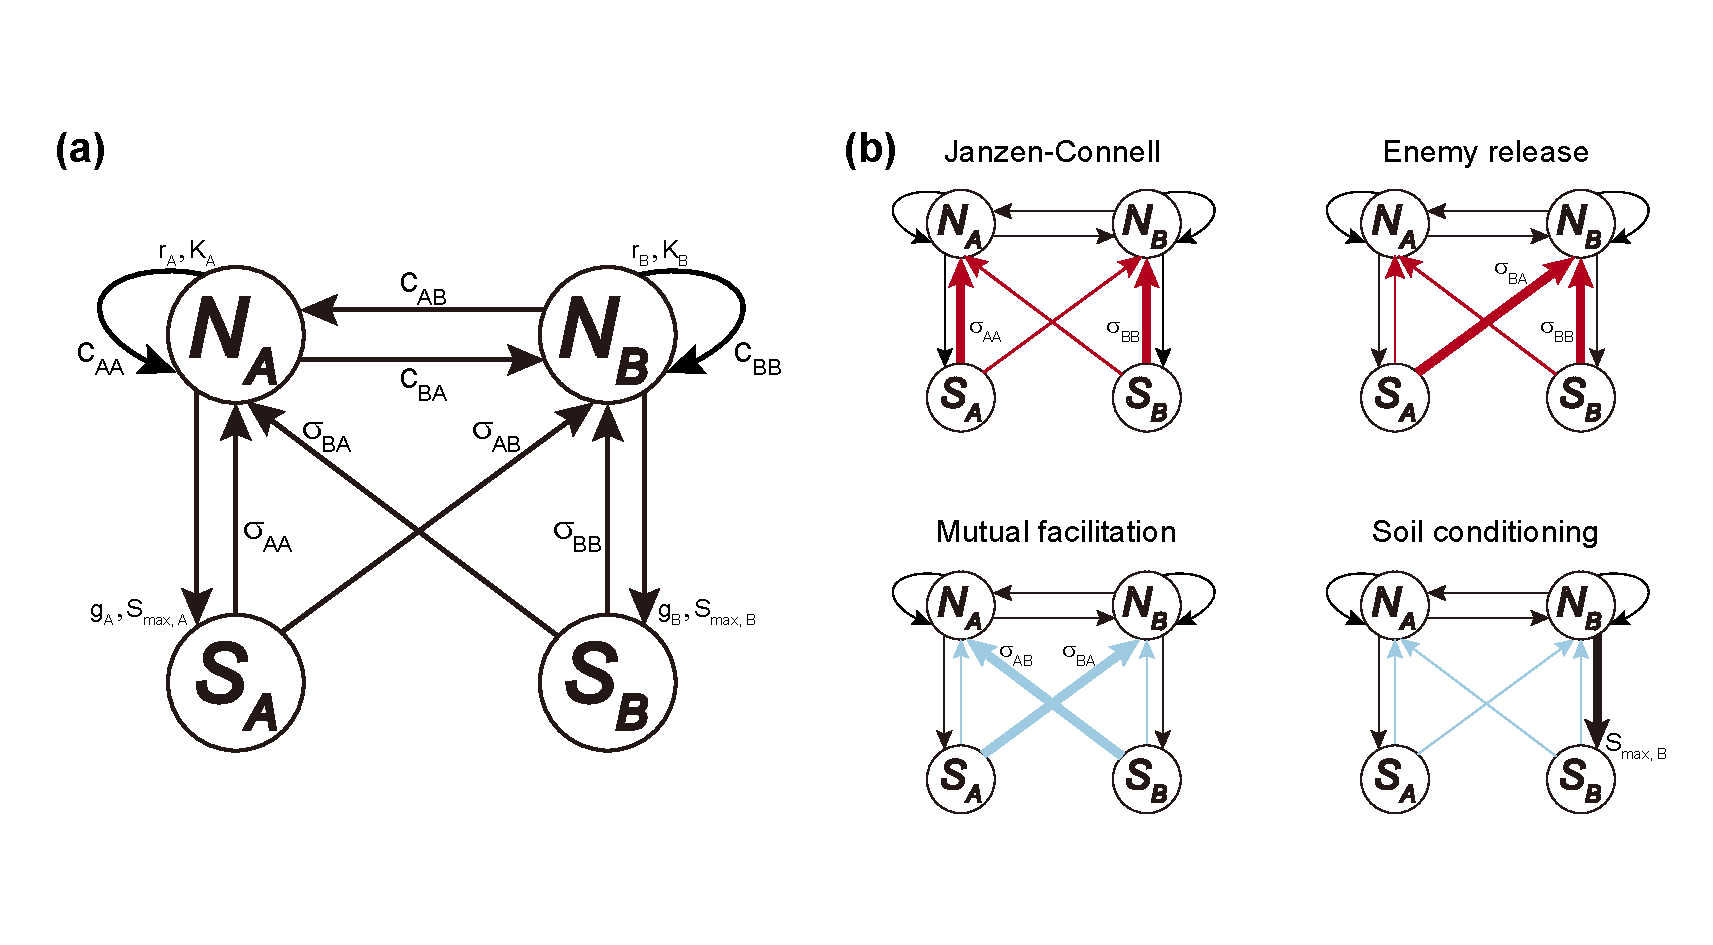
\includegraphics[width=16cm]{Chapter4/ModelFramework4_color_Revised2.pdf}}
	\caption[Conceptual framework for the plant--soil microbe interaction model.]
		{\hspace{1mm}Conceptual framework for the plant--soil microbe interaction model. (a) The model describes the dynamics of two plants (\textit{$N_{A}$} and \textit{$N_{B}$}) and the total density of their associated soil microbial communities (\textit{$S_{A}$} and \textit{$S_{B}$}), considering both plant--plant competition ($c_{ij}$) and plant--soil microbe interaction ($\sigma_{ij}$).  All arrows are labeled with corresponding model parameters; see main text for parameter definitions. (b) The four interaction scenarios analyzed in this study: Janzen--Connell (top left, varying $\sigma_{AA}$ and $\sigma_{BB}$); enemy release (top right, varying $\sigma_{BA}$ and $\sigma_{BB}$); mutual facilitation (bottom left, varying $\sigma_{AB}$ and  $\sigma_{BA}$); and differential soil conditioning (bottom right, varying $\phi_{B}$). Parameters varied in each scenario are highlighted with thick arrows. Soil microbial effects in the Janzen--Connell and enemy release scenario are pathogenic ($\sigma_{ij}<0$, dark red arrows), whereas in the mutual facilitation and differential soil conditioning scenario they are mutualistic ($\sigma_{ij}>0$, light blue arrows). Default parameter values are provided in Appendix C.4 (Table~\ref{table:Parameters}).}
	\label{fig:Framework}
\end{figure}



\clearpage
\begin{figure}[h!]
	\centering
	\makebox[\textwidth][c]{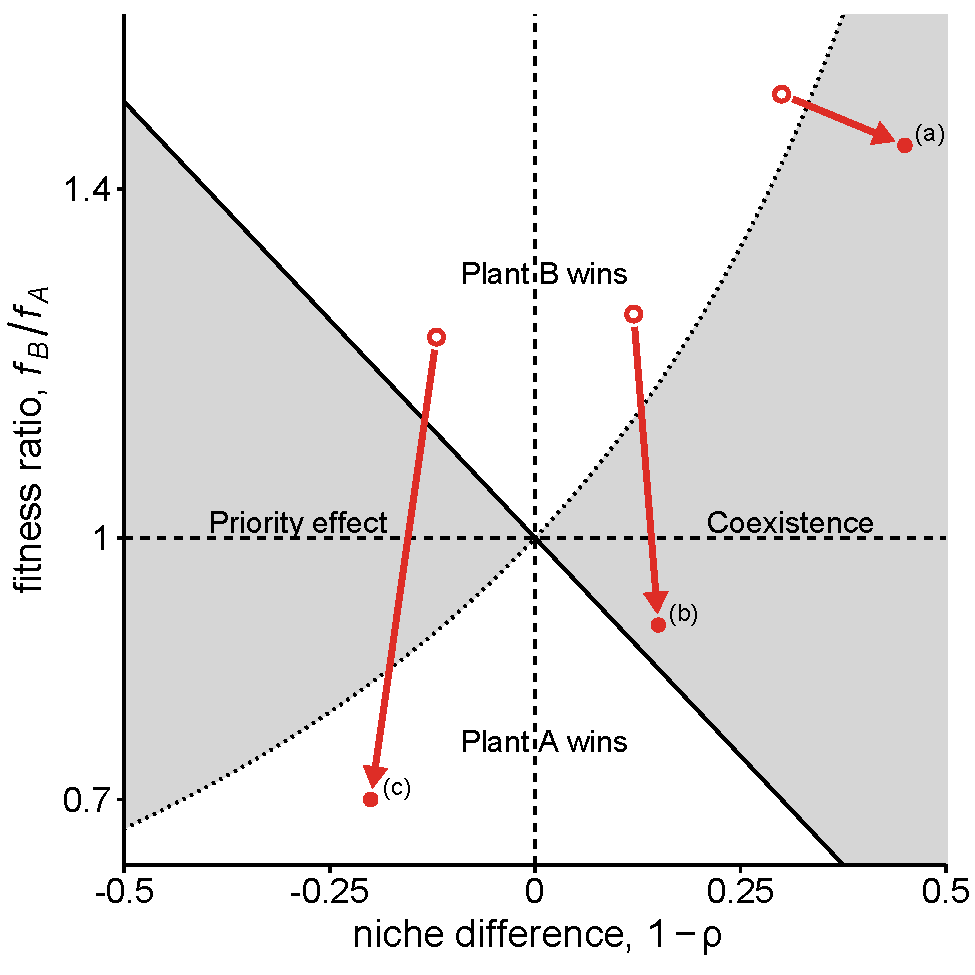
\includegraphics[width=11cm]{Chapter4/Conceptual2.pdf}}
	\caption[Potential effects of soil microbes on the outcome of plant competition, visualized on the parameter space of niche difference and fitness ratio.]
		{\hspace{1mm}Potential effects of soil microbes on the outcome of plant competition, visualized on the parameter space of niche difference ($1 - \rho$, x-axis) and fitness ratio ($f_{B}/f_{A}$, y-axis). The solid and dotted line represent the boundary where $f_{B}/f_{A}$ equals $\rho$ and $1/\rho$, respectively. The right and left gray shaded areas indicate the regions where coexistence and priority effects occur, respectively; the top and bottom white areas indicate where plant B or A is dominant, respectively. The red arrows demonstrate how soil microbes may alter the outcome of competition by (a) acting primarily as a stabilizing mechanism, (b) acting primarily as an equalizing mechanism, or (c) changing the identity of the dominant competitor. Open and solid circles represent competition in the absence and presence of soil microbes, respectively. This visualization was also used for the rest of our simulation results.}
	\label{fig:PopChessonSpace}
\end{figure}



\clearpage
\begin{figure}[h!]
	\centering
	\makebox[\textwidth][c]{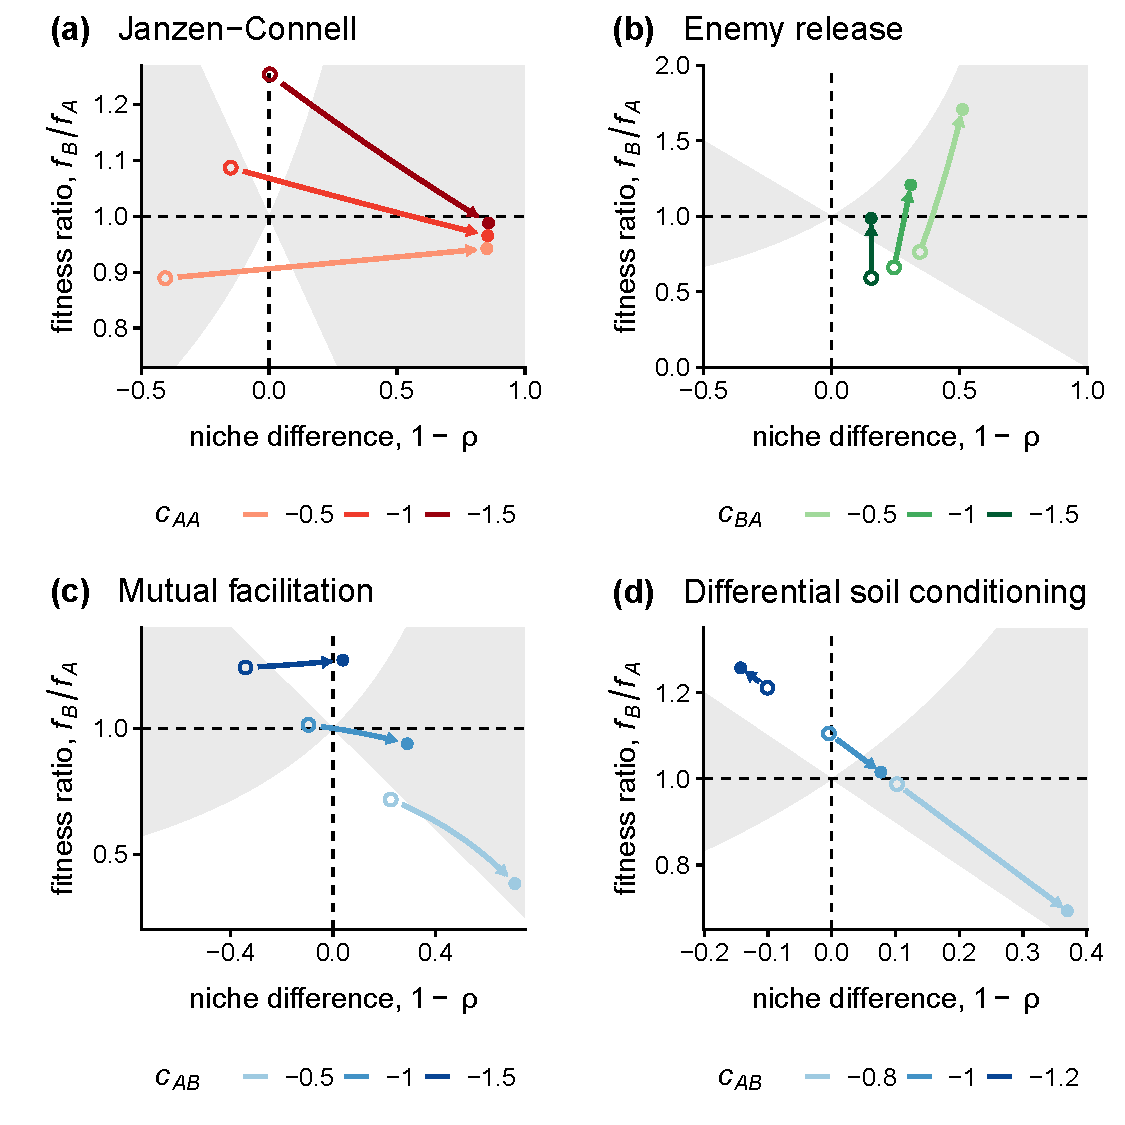
\includegraphics[width=14cm]{Chapter4/Translated_All_together.pdf}}
	\caption[Examples of how plant--soil microbe interactions and plant--plant competition together determine competition outcome.]
		{\hspace{1mm}Examples of how plant--soil microbe interactions and plant--plant competition together determine competition outcome. Four plant--soil microbe interaction scenarios were considered: (a) Janzen--Connell (varying $\sigma_{AA}$ and $\sigma_{BB}$), (b) enemy release (varying $\sigma_{BA}$ and $\sigma_{BB}$), (c) mutual facilitation (varying $\sigma_{AB}$ and  $\sigma_{BA}$), and (d) differential soil conditioning (varying $\phi_{B}$). For each scenario, arrows show how niche difference ($1 - \rho$, x-axis) and fitness ratio ($f_{B}/f_{A}$, y-axis) changed as we varied the strength of soil microbial effects ($\sigma_{ij}$) from weakest (open circles) to strongest (solid circles). To demonstrate its interactive effect with plant--plant competition, this trajectory is shown for different strengths of plant--plant competition ($c_{ij}$) ranging from weak (light colors) to strong (dark colors). Plant--plant competition coefficients that were shown here for each scenario are: (a) $c_{AA}$; (b) $c_{BA}$; (c) $c_{AB}$; and (d) $c_{AB}$. See Appendix C.4 for other plant--plant competition coefficients (Fig.~\ref{fig:Janzen_Connell_everything}--\ref{fig:Soil_Conditioning_everything}) and default parameter values (Table~\ref{table:Parameters}).}
	\label{fig:Scenario_Battleaxes}
\end{figure}



\clearpage
\begin{figure}[h!]
	\centering
	\makebox[\textwidth][c]{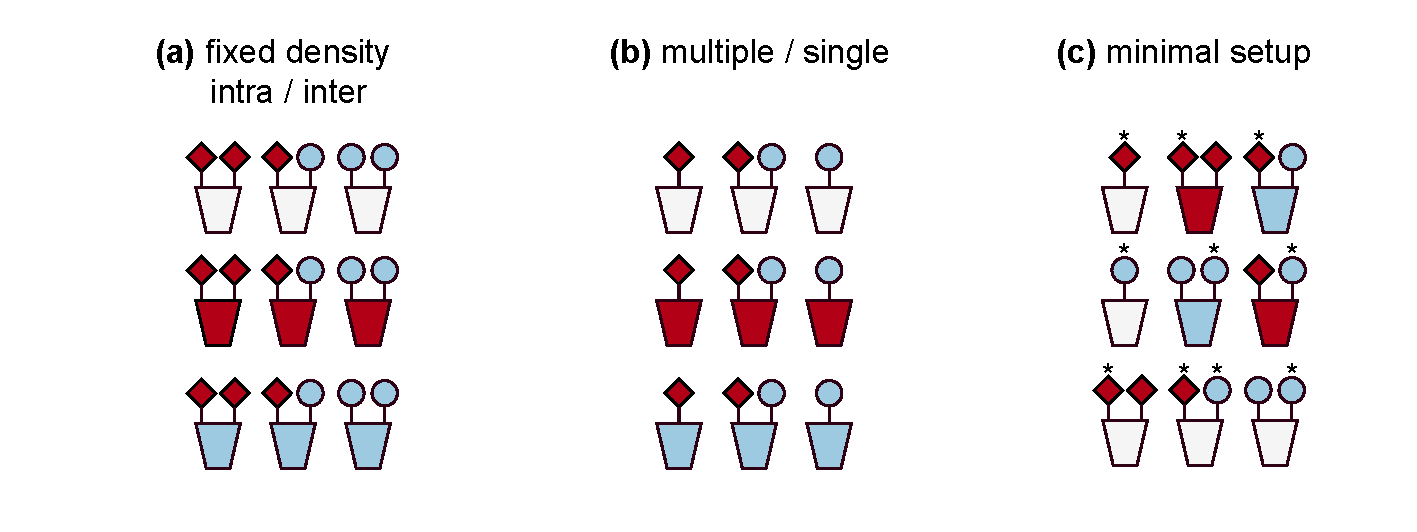
\includegraphics[width=16cm]{Chapter4/ExperimentSetupSmall_OnlyPots_Revised2_starred.pdf}}
	\caption[Experimental designs to quantify the effects of soil microbes on plant competitive outcome.]
		{\hspace{1mm}Experimental designs to quantify the effects of soil microbes on plant competitive outcome. (a) fixed-density intra/inter designs consisting of growing the focal plant in either intra- or inter-specific plant--plant competition; (b) multiple/single designs consisting of growing the focal plant either with or without interspecific plant--plant competition; (c) minimal experimental setup. Pots with different colors represent soils with different conditioning history: no conditioning history or sterile soil (white); conditioned by the diamond plant (dark red); conditioned by the circle plant (light blue). In the minimal setup, competition coefficients can be calculated from measurements of the plants marked with asterisks.}
	\label{fig:ExperimentSetup}
\end{figure}



\clearpage
\begin{figure}[h!]
	\centering
	\makebox[\textwidth][c]{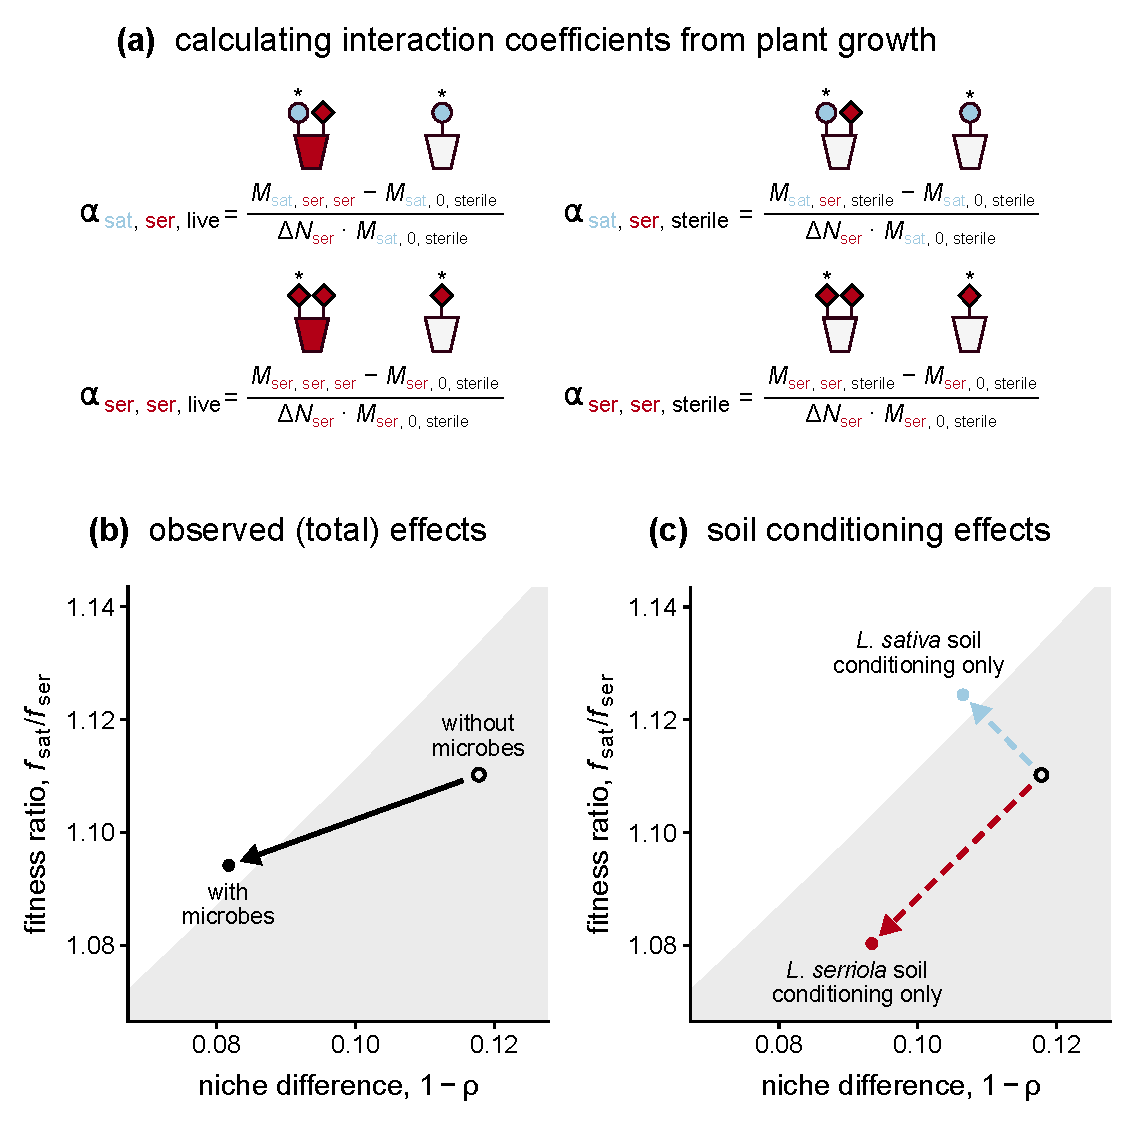
\includegraphics[width=15cm]{Chapter4/Aguilera_2panel_calculations_soil.pdf}}
	\caption[Applying modern coexistence theory to understand the effects of soil microbes on plant competitive outcome using data from \citet{Aguilera2017}as a case study.]
		{\hspace{1mm}Applying modern coexistence theory to understand the effects of soil microbes on plant competitive outcome using data from \citet{Aguilera2017}as a case study. (a) Calculating the competition coefficients representing the sensitivity of \textit{Lactuca sativa} (sat; blue) and \textit{Lactuca serriola} (ser; red) to \textit{L. serriola} in live and sterile soil. $M_{i,j,k}$ represents the biomass of species $i$ competing with species $j$ in soil cultivated by species $k$  (with $0$ indicating no competitor or no soil inoculum); $\Delta N_j$ represents the density of competitors of species $j$. Above each biomass term, we illustrate the corresponding experimental treatment and mark the measured individual with an asterisk. (b) Predicted effect of soil microbes (open circles: microbes absent; solid circles: microbes present) on the outcome of competition between \textit{L. sativa} and \textit{L. serriola}. Using competition coefficients calculated from empirical data, we applied our model to calculate niche difference and fitness ratio (see Box 2). The white region (upper left) indicates that \textit{L. sativa} outcompetes \textit{L. serriola}, whereas the gray region (lower right) indicates coexistence.}
	\label{fig:Aguilera2017Data}
\end{figure}



\clearpage 
\begin{flushleft}
\textbf{Box 4.1}
\end{flushleft}
\begin{infobox}[Separating the stabilizing and equalizing components]

To calculate the components of modern coexistence theory, we applied separation of timescales by assuming that soil microbe dynamics were sufficiently fast compared to plant population dynamics and that all dynamics occurred near equilibrium. In particular, this means that soil microbes reach their plant-determined carrying capacities without any time lag, and die instantly when the host plant dies. Under these conditions, we reduced our model (Eqns.~\ref{eq:SoilA}-\ref{eq:Nb}) to a two-species Lotka--Volterra model (see Appendix C.2), with the following interaction coefficients:

\begin{equation}
\alpha_{ij} = c_{ij} + \sigma_{ij}\phi_{j} .
\tag{4.5}\label{eq:alpha}
\end{equation}

Here, $\alpha_{ij}$ represents the net competitive effect of species $j$ on $i$ and $i$ and $j = A$ or $B$. Importantly, we can observe that net competition consists of two terms: (1) plant--plant competition not related to soil microbes, $c_{ij}$, and (2) soil microbial effects, summarized as $\sigma_{ij}\phi_{j}$.
We assumed plant--plant interactions are competitive ($c_{ij} < 0$) and plant--soil microbe interactions can be either detrimental ($\sigma_{ij} < 0$) or beneficial ($\sigma_{ij} > 0$). Note that when microbes have no effect on plants ($\sigma_{ij}$ or $\phi_{i} = 0$), the model simplifies to pure Lotka--Volterra competition. In addition, if the soil microbes have a very strong positive effect, $\alpha_{ij}$ becomes greater than zero and the plant populations grow towards infinite population size without other regulatory forces.
\par


% Separating ND and FD from the PSF model -- Using Chesson's formula
After transforming the model, we quantified niche overlap and fitness ratio between the two plants using formulas derived specifically for two-species Lotka--Volterra models \citep{Chesson1990, Chesson2008b, Chesson2013ecosys}. Under this formalization, stabilizing mechanisms represent processes that decrease niche overlap ($\rho$, or increase niche difference, $1-\rho$). Here, $\rho$ is the magnitude of difference in inter- to intra-specific interaction coefficients, i.e., $\rho = \sqrt{\frac{\alpha_{BA}\alpha_{AB}}{\alpha_{AA}\alpha_{BB}}}$. Equalizing mechanisms, on the other hand, represent processes that reduce the fitness ratio, which is defined as $\frac{f_{B}}{f_{A}} = \sqrt{\frac{\alpha_{AA}\alpha_{AB}}{\alpha_{BB}\alpha_{BA}}}$. Following these definitions, we derived the niche overlap and fitness ratio between $N_{A}$ and $N_{B}$ as:
\begin{equation}
\rho = \sqrt{\frac{\left ( c_{BA} + \sigma_{BA}\phi_{A} \right )
				   \left ( c_{AB} + \sigma_{AB}\phi_{B} \right )}
				  {\left ( c_{AA} + \sigma_{AA}\phi_{A} \right )
				   \left ( c_{BB} + \sigma_{BB}\phi_{B} \right )}}
\tag{4.6}\label{eq:ND}
\end{equation}
\begin{equation}
\frac{f_{B}}{f_{A}} = \sqrt{\frac{\left ( c_{AA} + \sigma_{AA}\phi_{A} \right )
								  \left ( c_{AB} + \sigma_{AB}\phi_{B} \right )}
								 {\left ( c_{BB} + \sigma_{BB}\phi_{B} \right )
								  \left ( c_{BA} + \sigma_{BA}\phi_{A} \right )}} .
\tag{4.7}\label{eq:FR}
\end{equation}
\end{infobox}



\clearpage
\begin{flushleft}
	\textbf{Box 4.2}
\end{flushleft}
\begin{infobox}[Visualizing the niche difference--fitness ratio parameter space]

In this study, we visualize our simulation results on the parameter space defined by the niche difference ($1-\rho$) and fitness ratio ($f_{B} / f_{A}$) between the two species. Here, we use figure~\ref{fig:PopChessonSpace} as an illustrative example to demonstrate how to interpret our results. The solid linear and dotted curvilinear black lines denote the boundary where fitness ratio is equal to niche overlap ($\rho$) and the inverse of niche overlap ($1 / \rho$), respectively. These two boundaries partition the parameter space into four distinct regions, representing different outcomes of competition. If the two species differ too greatly in fitness relative to their niche difference, one species outcompetes the other (upper and lower white regions). When the niche difference is positive, stable coexistence occurs if the fitness ratio is not too extreme (right gray region). When niche difference is negative, priority effects may occur (left gray region), where community composition depends on which plant arrives first \citep{Mordecai2011, KeLetten2018}.
\par


The pathways shown in Figure~\ref{fig:PopChessonSpace} illustrate how soil microbes might alter competitive outcomes. For example, soil microbes may promote coexistence by primarily affecting niche difference (a stabilizing mechanism, arrow a in Fig.~\ref{fig:PopChessonSpace}) or fitness ratio (an equalizing mechanism, arrow b Fig.~\ref{fig:PopChessonSpace}). Soil microbes may also flip the competitive hierarchy by changing the identity of the dominant competitor (arrow c in Fig.~\ref{fig:PopChessonSpace}).
Note that since microbe-mediated parameters make up part of the phenomenological interaction coefficients (Eqn.~\ref{eq:alpha}), varying their strength would simultaneously affect both niche difference and fitness ratio.
The only exception being the special case where a pair of $\sigma_{ij}$ varied in a way that maintained the value of either Eqns.~\ref{eq:ND} or \ref{eq:FR}.
In general, however, plant--soil interactions would predominantly affect either the stabilizing or equalizing components depending on the specific interaction network between plants and soil microbes (see section \textit{Synthesizing microbial effects on plant coexistence}).
\end{infobox}